\section{Object Oriented systems}


%\todo[inline]{leer el paper de historia de poo, en la 2da pagina}
%\cite{Wegner:1987}

Many autors formulate precise 
definition of \gls{O-O} paradigm 
\cite{Rentsch:1982} 
\cite{Pascoe:1986}
\cite{Nygaard:1986}
\cite{Madsen:1988}, 
and the definition of Lastly, Wegner 
\cite{Wegner:1987} has been 
the most widely 
accepted \cite{Capretz:2003}. Wegner defines 
the \gls{O-O} paradigm in terms of objects, 
classes and inheritance.

\emph{
	``Objects are autonomous entities 
	that respond to messages or operations and share 
	a state. Classes classify objects by their common 
	operations. Inheritance serves to classify classes by 
	their shared behavior. Data abstraction hides the 
	representation of data and the implementation of 
	operations'' 
}\cite{Wegner:1987}. That is: 

\begin{center}
	object oriented = objects + classes + inheritance
\end{center}
In the next sections theses concepts are explained.

%This paradigm is useful to develop scalable, 
%consistent and reliable software systems 
%organizing the code to create objects. 
The O-O system programming metodology 
defines an approach to code organization 
for objects creation. 
The objects store the data and 
have their own behabiour with a 
particular information grouping 
by common functionality and common 
information structures. 
O-O systems benefits 
to bundle actions together, 
manage a few quantity of variables rather 
than multiples ones, 
organizing the 
common behavior together and 
structure programs in a way that
matches closely 
the real world \cite{Adobe:AS3man2008}. 

The figure \ref{fig:real-world-objets-represented} shows  
\todo{
	esta figura esta incompleta, deberia conseguir unas
	buenas fotos (en itaipu hay muchas fotos lindas y 
	originales) de estos equipamientos
	electricos de la Itaipu y colocar unas 
	flechitas que unen a estos 
	diagramas con los objetos reales
	y palabras indicativas\ldots
} 
a real world substation, their equipments, 
and the virtual substation  
software engineering representation 
through the class \emph{tSubstation} that 
responds with the same behabiour as in 
the real world, 
but running by software.


\begin{figure}
  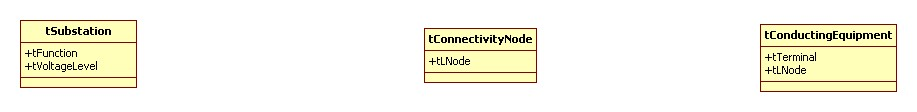
\includegraphics[width=1.0\textwidth]{chapters/ch-oop/figures/real-word-objets-represented}
  \caption{Real world object and their representation in software engineering}
  \label{fig:real-world-objets-represented}
\end{figure}

